\documentclass[8pt,landscape]{article}
\usepackage[a4paper,top=0.5cm,bottom=0.5cm,left=0.5cm,right=0.5cm]{geometry}

\usepackage[ngerman]{babel}
\usepackage{graphicx}
\usepackage[utf8]{inputenc}
\usepackage{amsfonts}
\usepackage{multicol}
\setlength\parindent{0ex}
\usepackage{amsmath}
\setlength{\columnsep}{10mm}
\usepackage{blindtext}
\usepackage{paralist}
\usepackage{bbm} % Natural numbers etc.

% Use compactitem.



% -------------- Beginning of Document ---------------. 
\begin{document}


\renewcommand{\labelitemi}{--}
%\setlist{noitemsep}
\pagestyle{empty}
\raggedright
\setlength{\columnsep}{2mm}
\setlength{\columnseprule}{0.1mm}
\begin{multicols}{3}
\title{\textbf{Autonomous Mobile Robots}}
\author{Fabian Blöchliger}
\date{Spring Semester 2016}
\maketitle


\section{Introduction and Motivation}

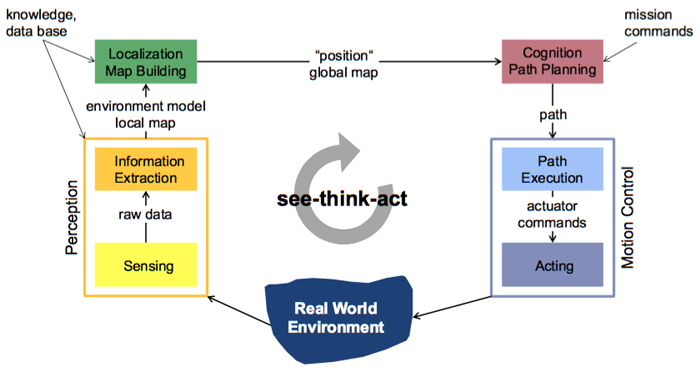
\includegraphics[width=\columnwidth]{img/1_SeeThinkAct.png}

\section{Locomotion Concepts}

\blindtext[3]

\section{Mobile Robot Kinematics}

\blindtext[3]

\section{Perception I}

\blindtext[3]

\section{Perception II}

\blindtext[3]

\section{Perception III}

\blindtext[3]

\section{Perception IV}

\blindtext[3]

\section{Localization I}

\blindtext[3]

\section{Localization II}

\blindtext[3]

\section{SLAM I}

\blindtext[3]

\section{SLAM II}

\blindtext[3]

\section{Planning I}

\blindtext[3]

\section{Planning II}

\blindtext[3]





\end{multicols}

% -------------- End of Document ---------------------. 
\end{document}
